\section{Learning Curves}
\begin{frame}{Learning Curves}

\centering
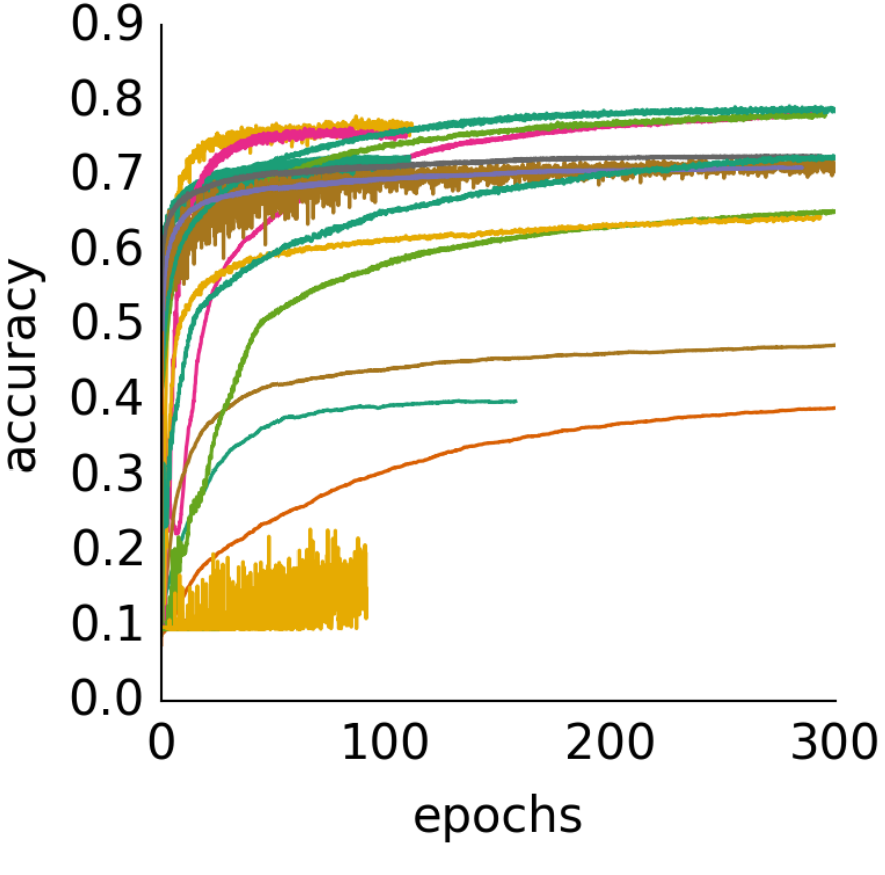
\includegraphics[width=0.4\textwidth]{w07_hpo_grey_box/images/learningcurve/learning_curves.png}

Exemplary learning curves of training deep neural networks\\
Many ML algorithms iteratively optimize a (loss) function

\end{frame}
%-----------------------------------------------------------------------

%-----------------------------------------------------------------------
\begin{frame}{Learning Curve Predictions}

\centering
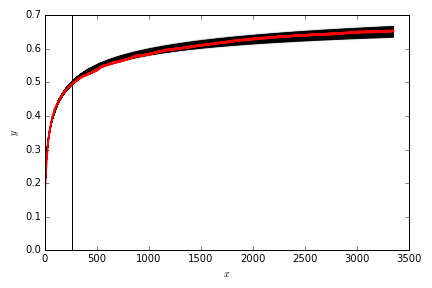
\includegraphics[width=0.5\textwidth]{w07_hpo_grey_box/images/learningcurve/learning_curve_single_pred.jpg}

\begin{enumerate}
  \item Observe learning curve for the first $n$ steps (here $n=250$)
  \pause
  \item \alert{Extrapolation}: fit parametric model on partial learning curve to predict remaining learning curve
  \pause
  \begin{itemize}
      \item Various models can be used (see following slides) 
  \end{itemize}
  
 % Which model to use? E.g.,
 % \begin{itemize}
%	\item Parametric density models: give table with equations
%	\item Neural network with learning curve layer
%	\item Recurrent neural network
%%    \item Good model depends on shape of curve $\to$ e.$\,$g., depends on optimizer  
%%    \item[$\leadsto$] combination of several models
%  \end{itemize}
  
\end{enumerate}

\end{frame}
%-----------------------------------------------------------------------

%-----------------------------------------------------------------------
\begin{frame}{Learning Curves: Early Termination}

\centering
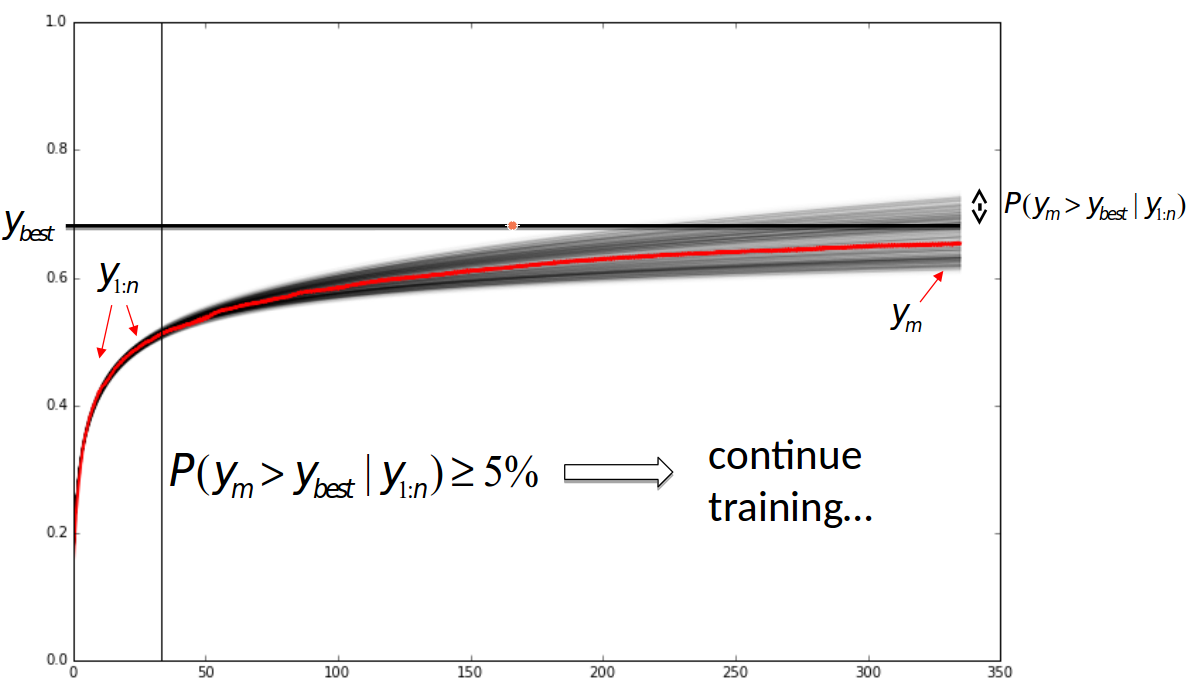
\includegraphics[width=0.8\textwidth]{w07_hpo_grey_box/images/learningcurve/learning_curve_dec.png}

$\rightarrow$ need for \alert{probabilistic predictions / quantification of uncertainty}

\end{frame}
%-----------------------------------------------------------------------
%-----------------------------------------------------------------------
\begin{frame}{Learning Curves: Early Termination}

\centering
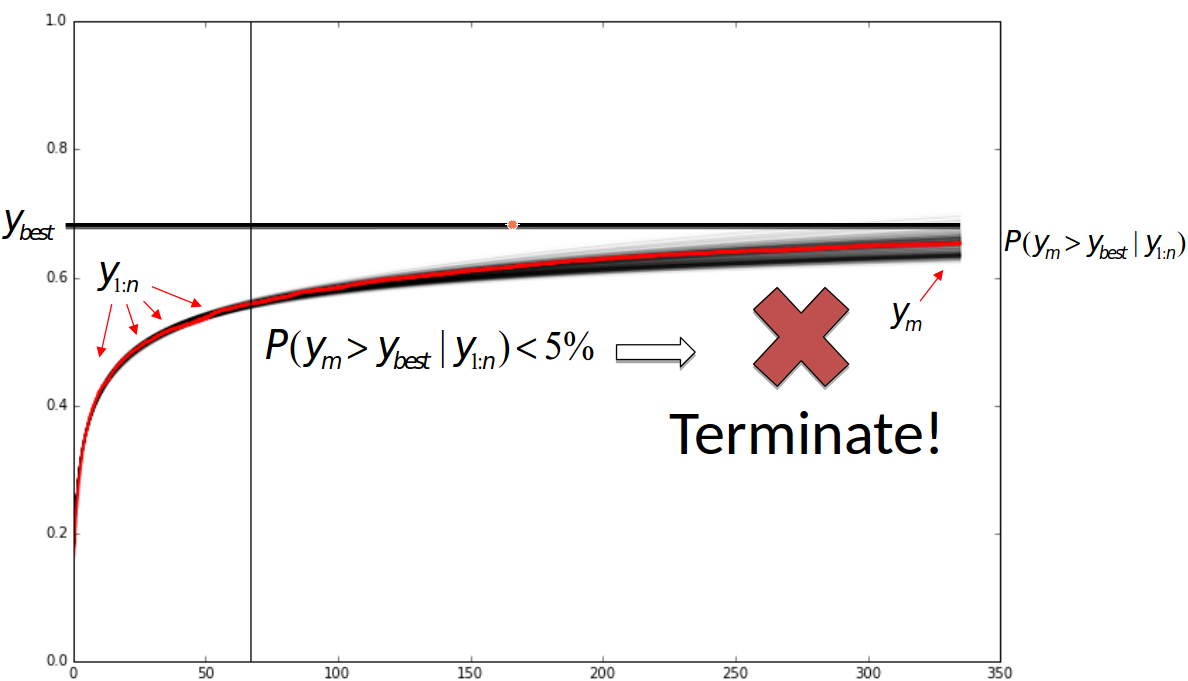
\includegraphics[width=0.8\textwidth]{w07_hpo_grey_box/images/learningcurve/learning_curve_dec2.png}

$\rightarrow$ need for \alert{probabilistic predictions / quantification of uncertainty}

\end{frame}
%-----------------------------------------------------------------------

%-----------------------------------------------------------------------
\begin{frame}{Parametric Learning Curves}

\myit{
	\item Use a parametric model $f_k$ with parameters $\boldsymbol{\theta}$ to model performance at step $t$ as:
	\alert{$y_t = f_k(t|\boldsymbol{\theta}) + \epsilon$}, with $\epsilon \sim \mathcal{N}(0, \sigma^2)$.
\pause
	\item Linear combination of $K=11$ parametric types of models:
	\alert{$f_{comb}(t|\bm{\xi}) = \sum_{k=1}^K w_k f_k(t|\boldsymbol{\theta}_k)$},
where $\bm{\xi} = (w_1, \dots, w_{K}, \boldsymbol{\theta}_1, \dots, \boldsymbol{\theta}_{K}, \sigma^2)$
%	\item MSc Thesis in my group, 2015
}
\begin{center}
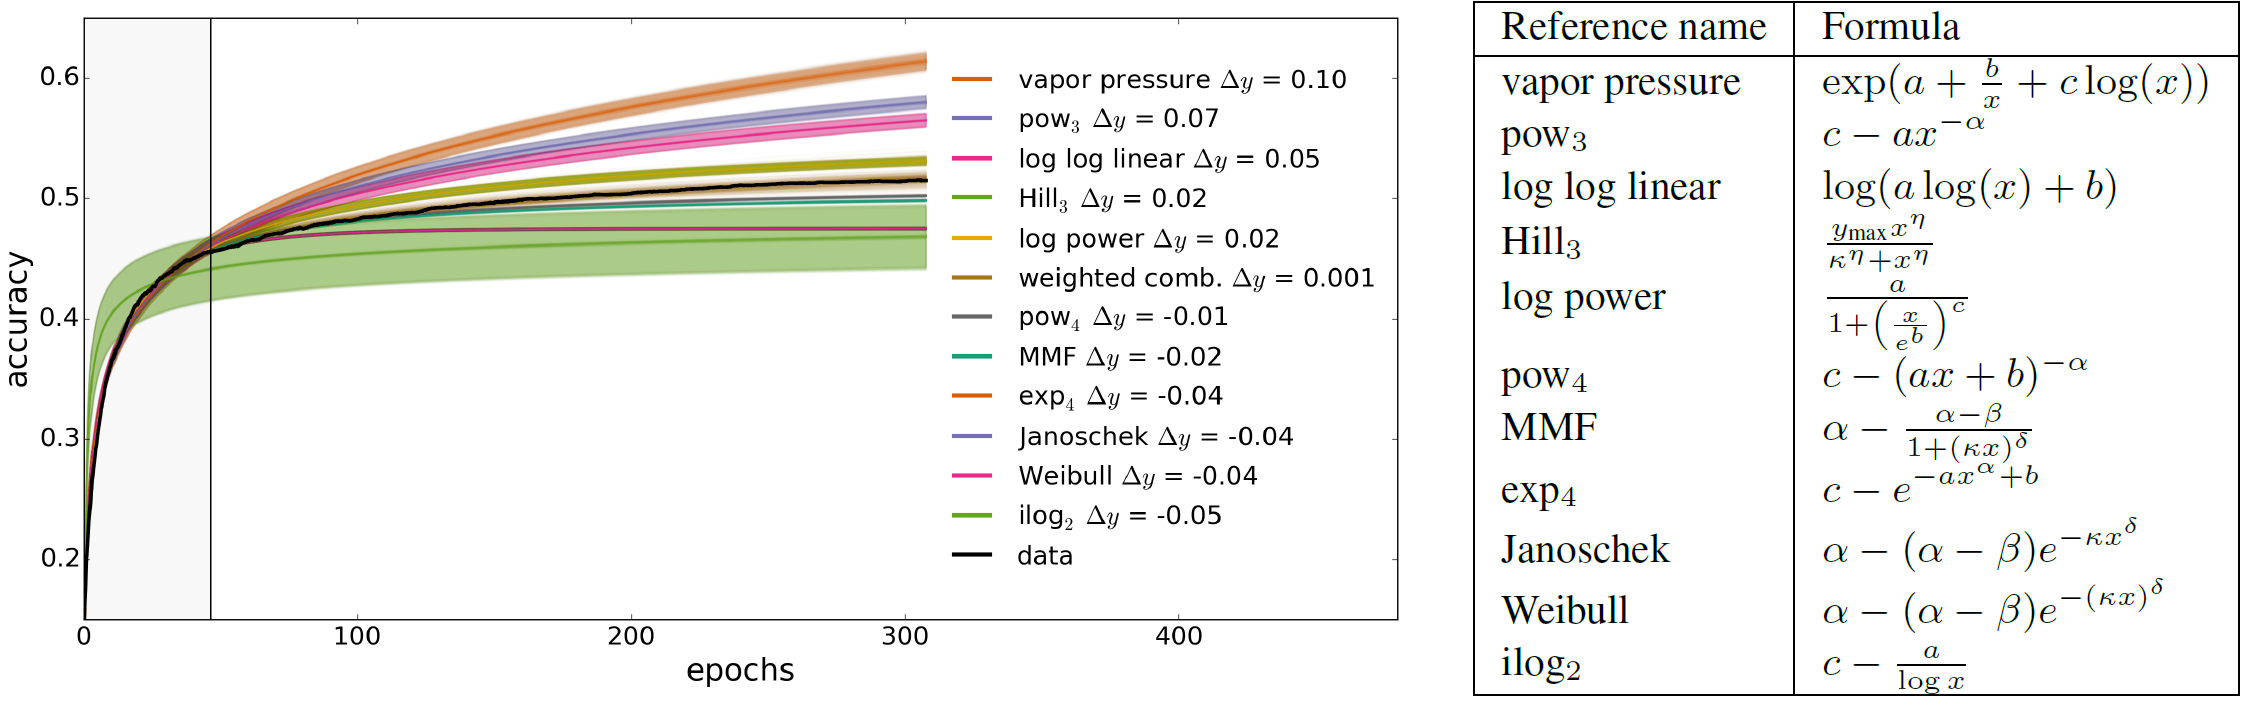
\includegraphics[width=0.9\textwidth]{w07_hpo_grey_box/images/learningcurve/Domhan_types_of_curves.png}\\
\scriptsize{$K=11$ parametric families for modelling learning curves}
\end{center}

\pause
\myit{
	\item Use Markov Chain Monte Carlo sampling of $\bm{\xi}$ to obtain uncertainties
}

\end{frame}
%-----------------------------------------------------------------------

%-----------------------------------------------------------------------
\begin{frame}{Predictive Termination}

{
\begin{center}
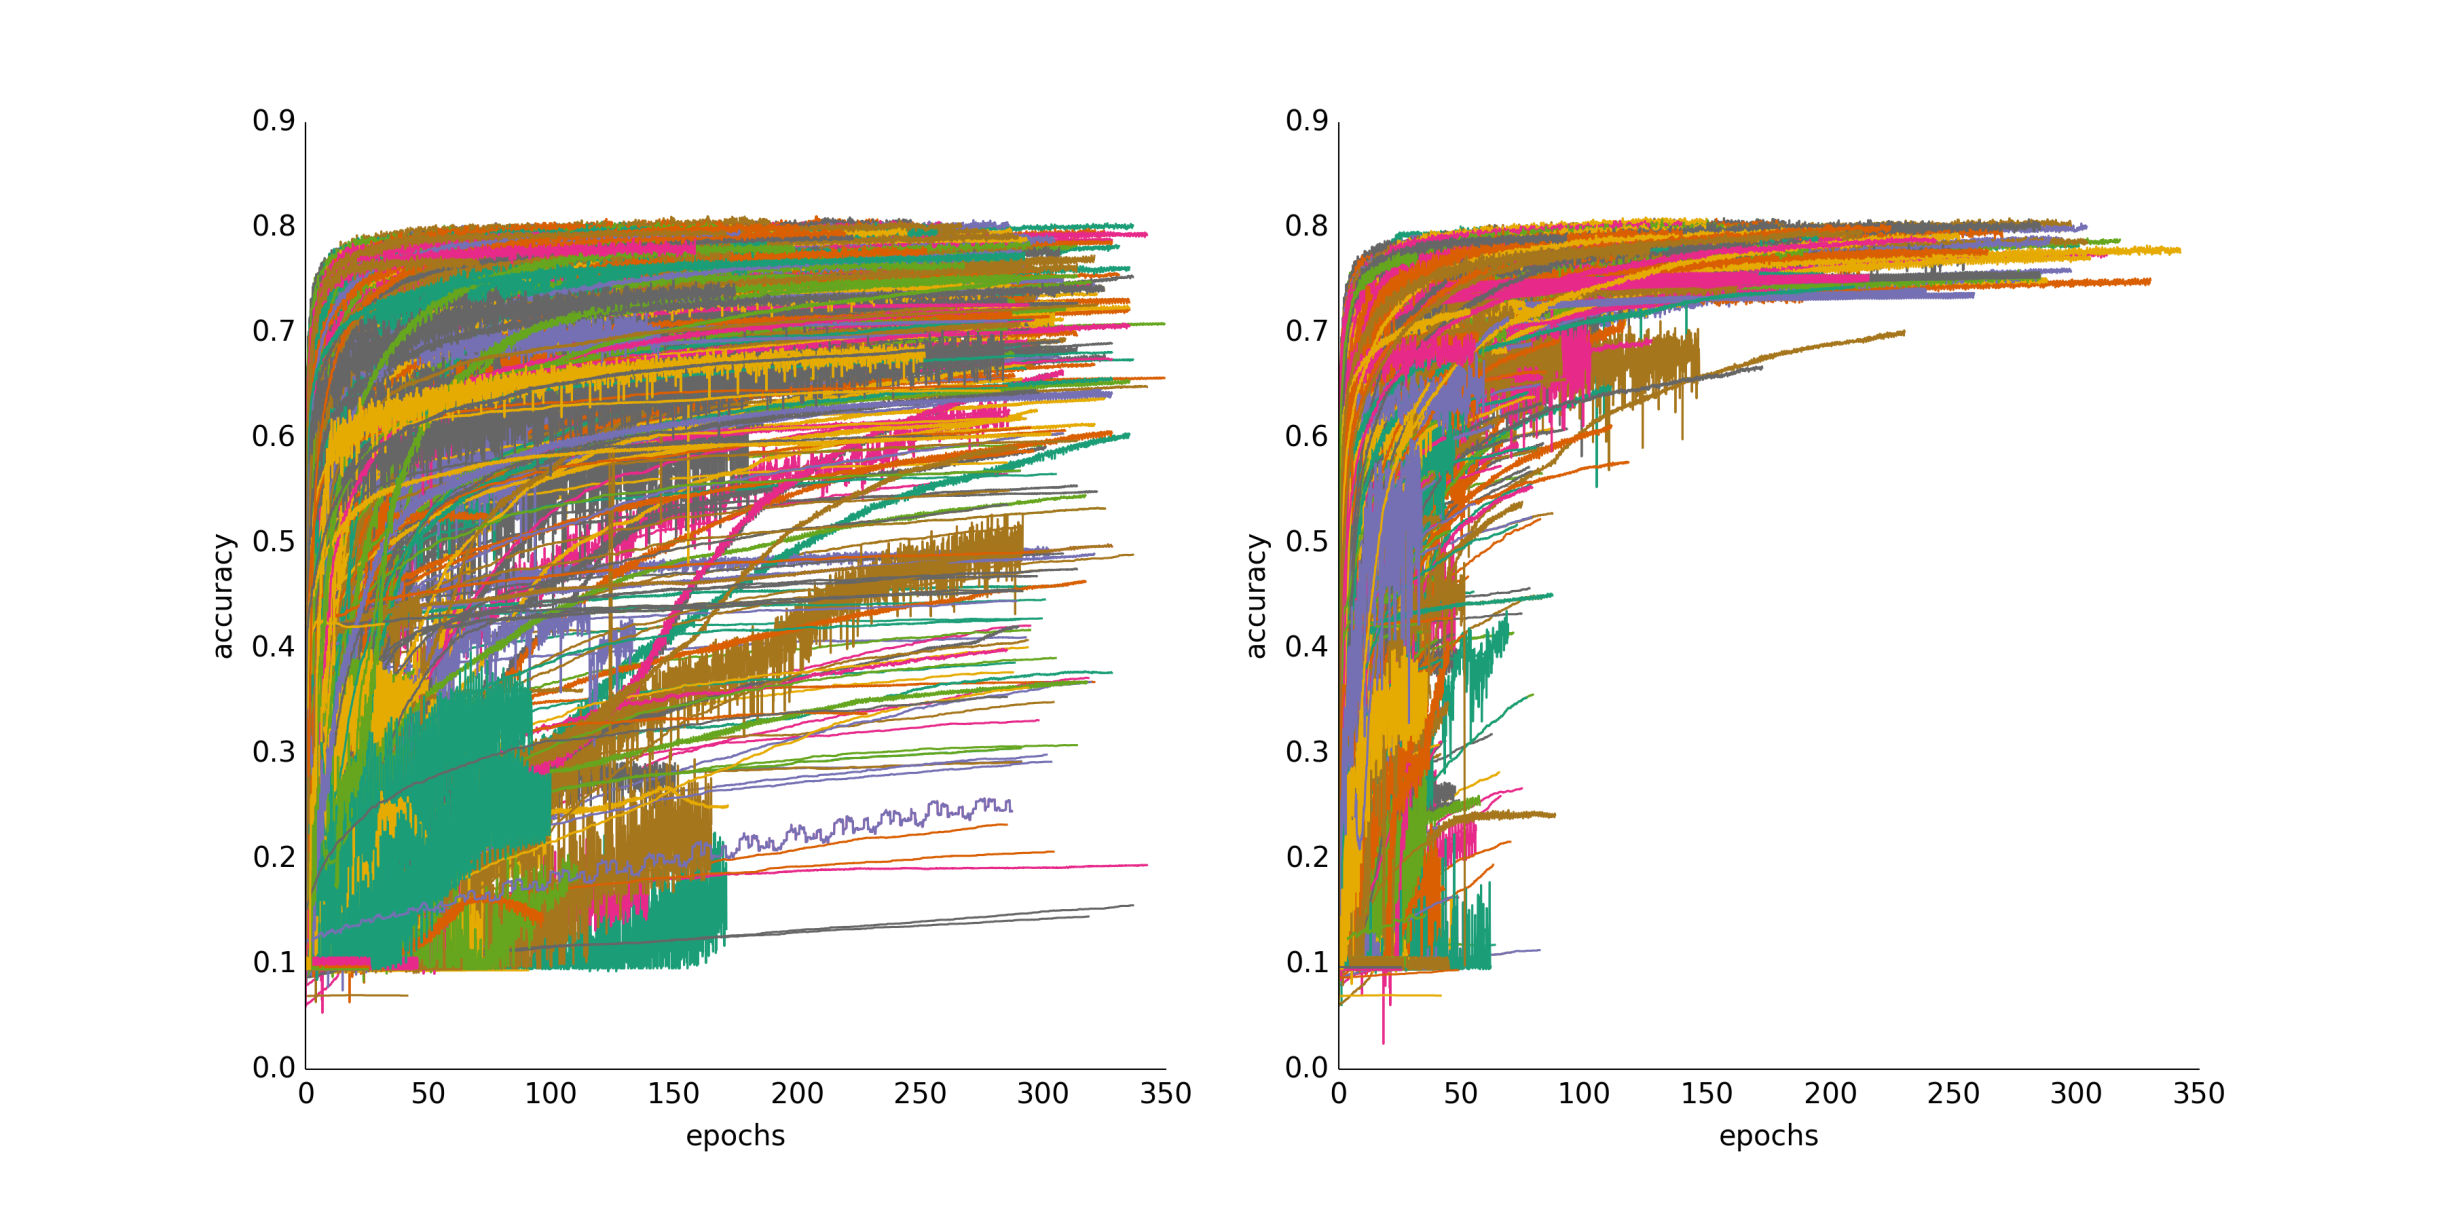
\includegraphics[width=0.9\textwidth]{w07_hpo_grey_box/images/learningcurve/learning_curve_tuning.jpg}

All learning curves vs. learning curves with early termination
\end{center}
}




\end{frame}
%-----------------------------------------------------------------------
%-----------------------------------------------------------------------
\begin{frame}{Predictive Termination}

{
\begin{center}
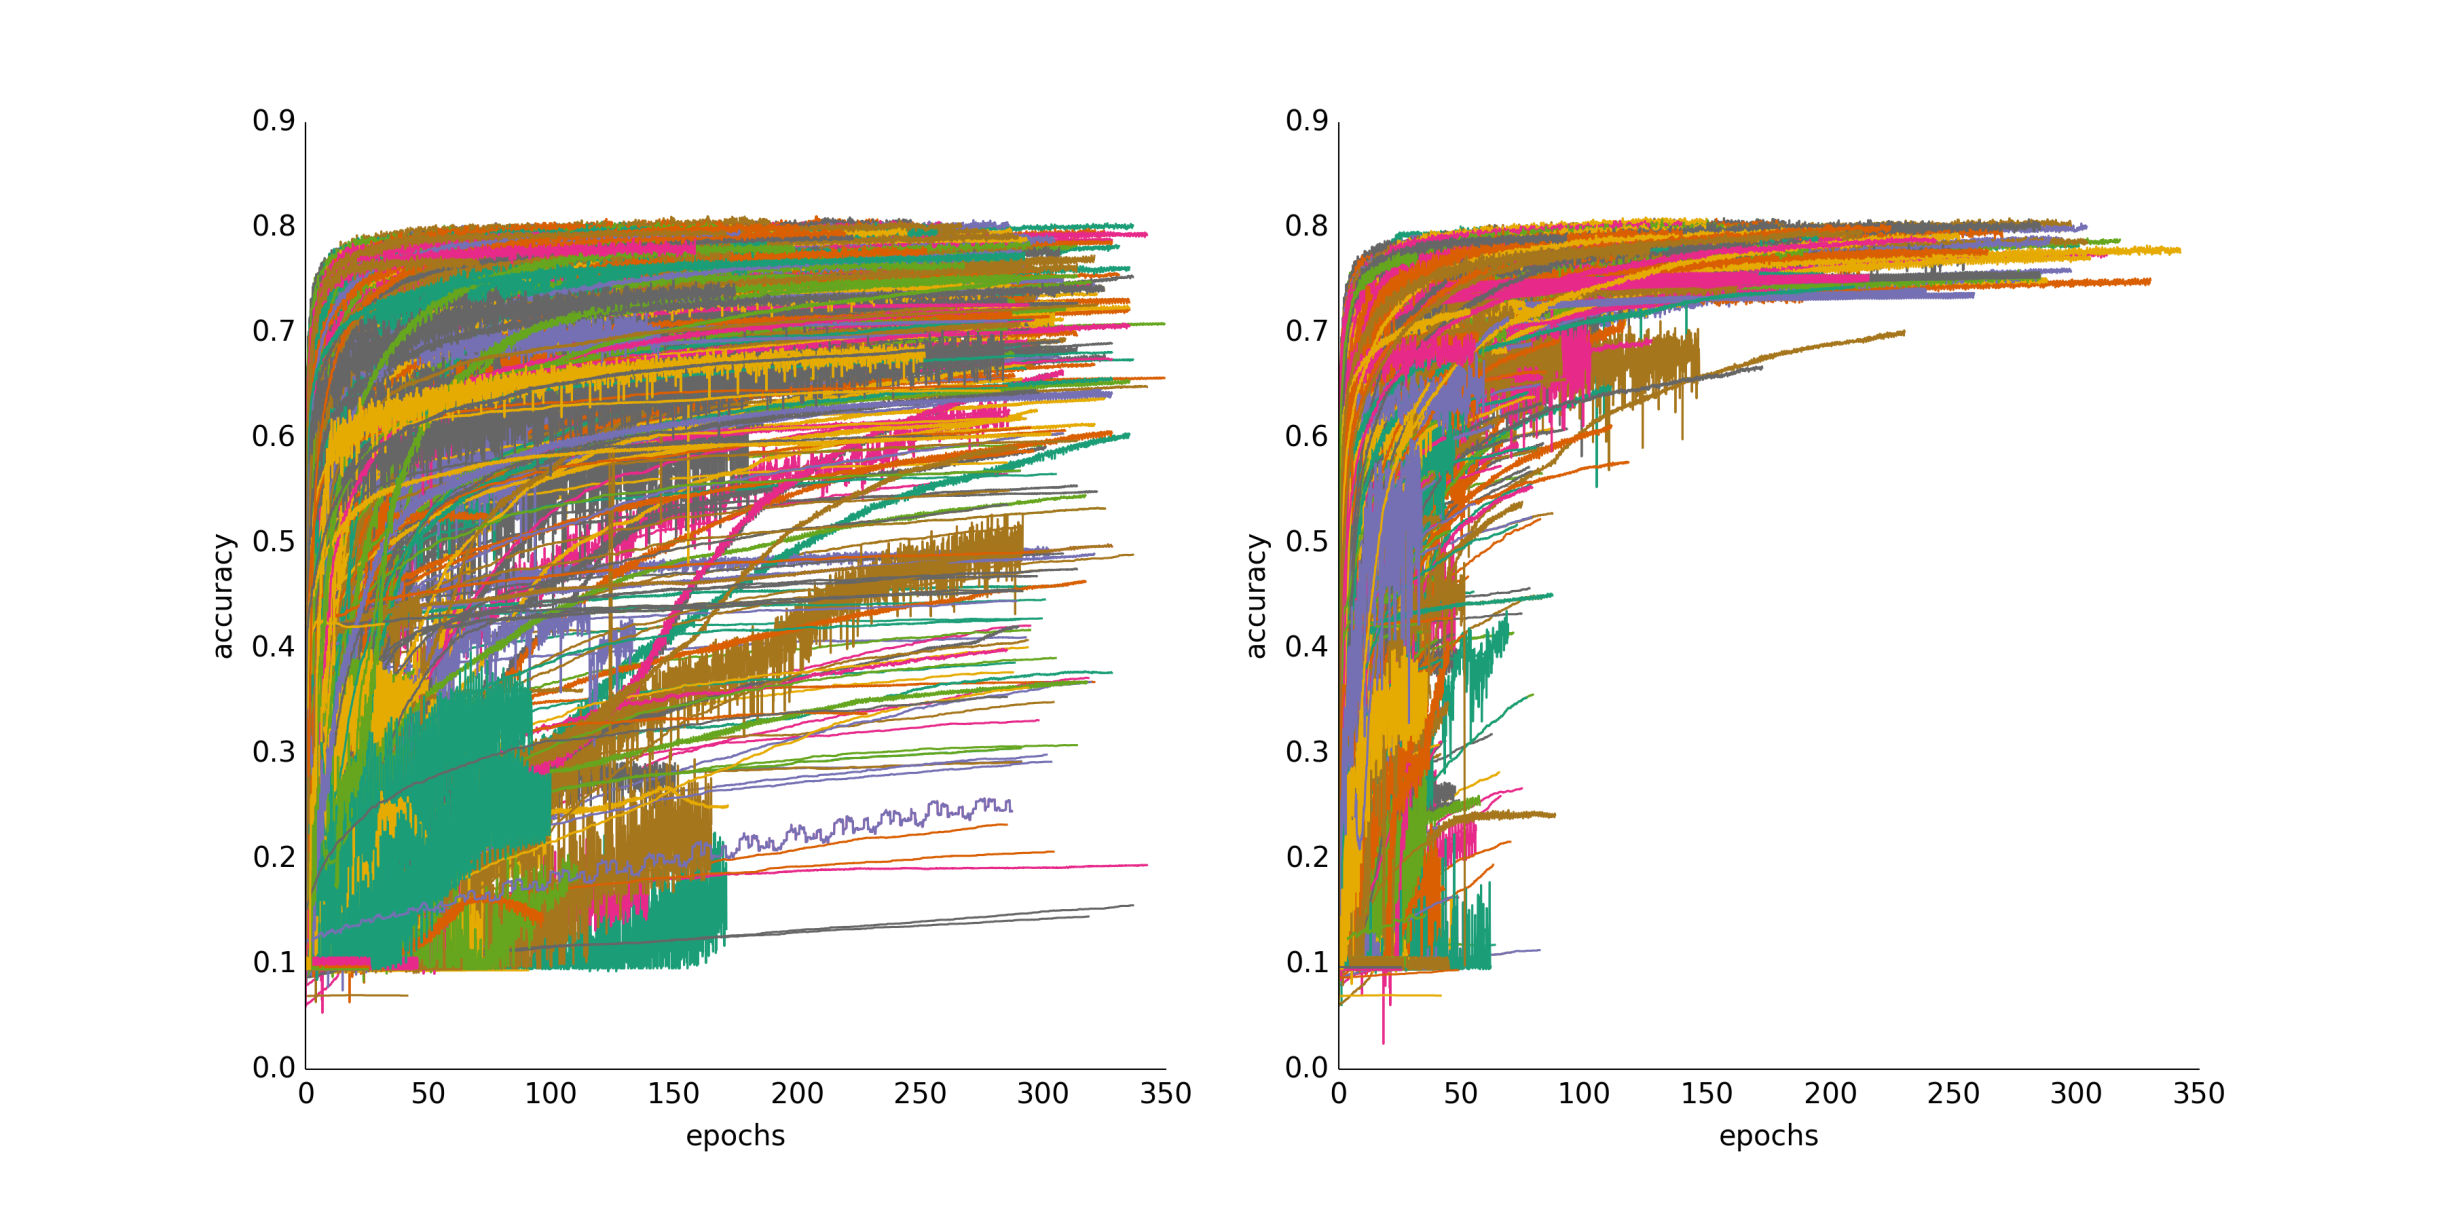
\includegraphics[width=0.5\textwidth]{w07_hpo_grey_box/images/learningcurve/learning_curve_tuning.jpg}

All learning curves vs. learning curves with early termination
\end{center}
}
\myit{
	\item Disadvantages of this model?
\pause
	\myit{
		\item Relies on manually-selected parametric families of curves
		\item Does not take into account hyperparameters used 
		\myit{
			\item[$\rightarrow$] can't learn across hyperparameters
		}
		\item Does not even learn across curves; simply extrapolates one at a time
%		\item Cannot quickly integrate new information from extending the curve
	}
}

\end{frame}
%-----------------------------------------------------------------------
\begin{frame}{Freeze-Thaw Bayesian Optimization}

\myit{
	\item Use a Gaussian process with inputs $\conf$ and $t$; special kernel for $t$
	\item For $N$ configurations and $T$ epochs each: $O(N^3 t^3)$ $\rightarrow$ approximation
	\item Iteratively: either extend existing configuration or try new one
\pause
	\item Result for probabilistic matrix factorization:
	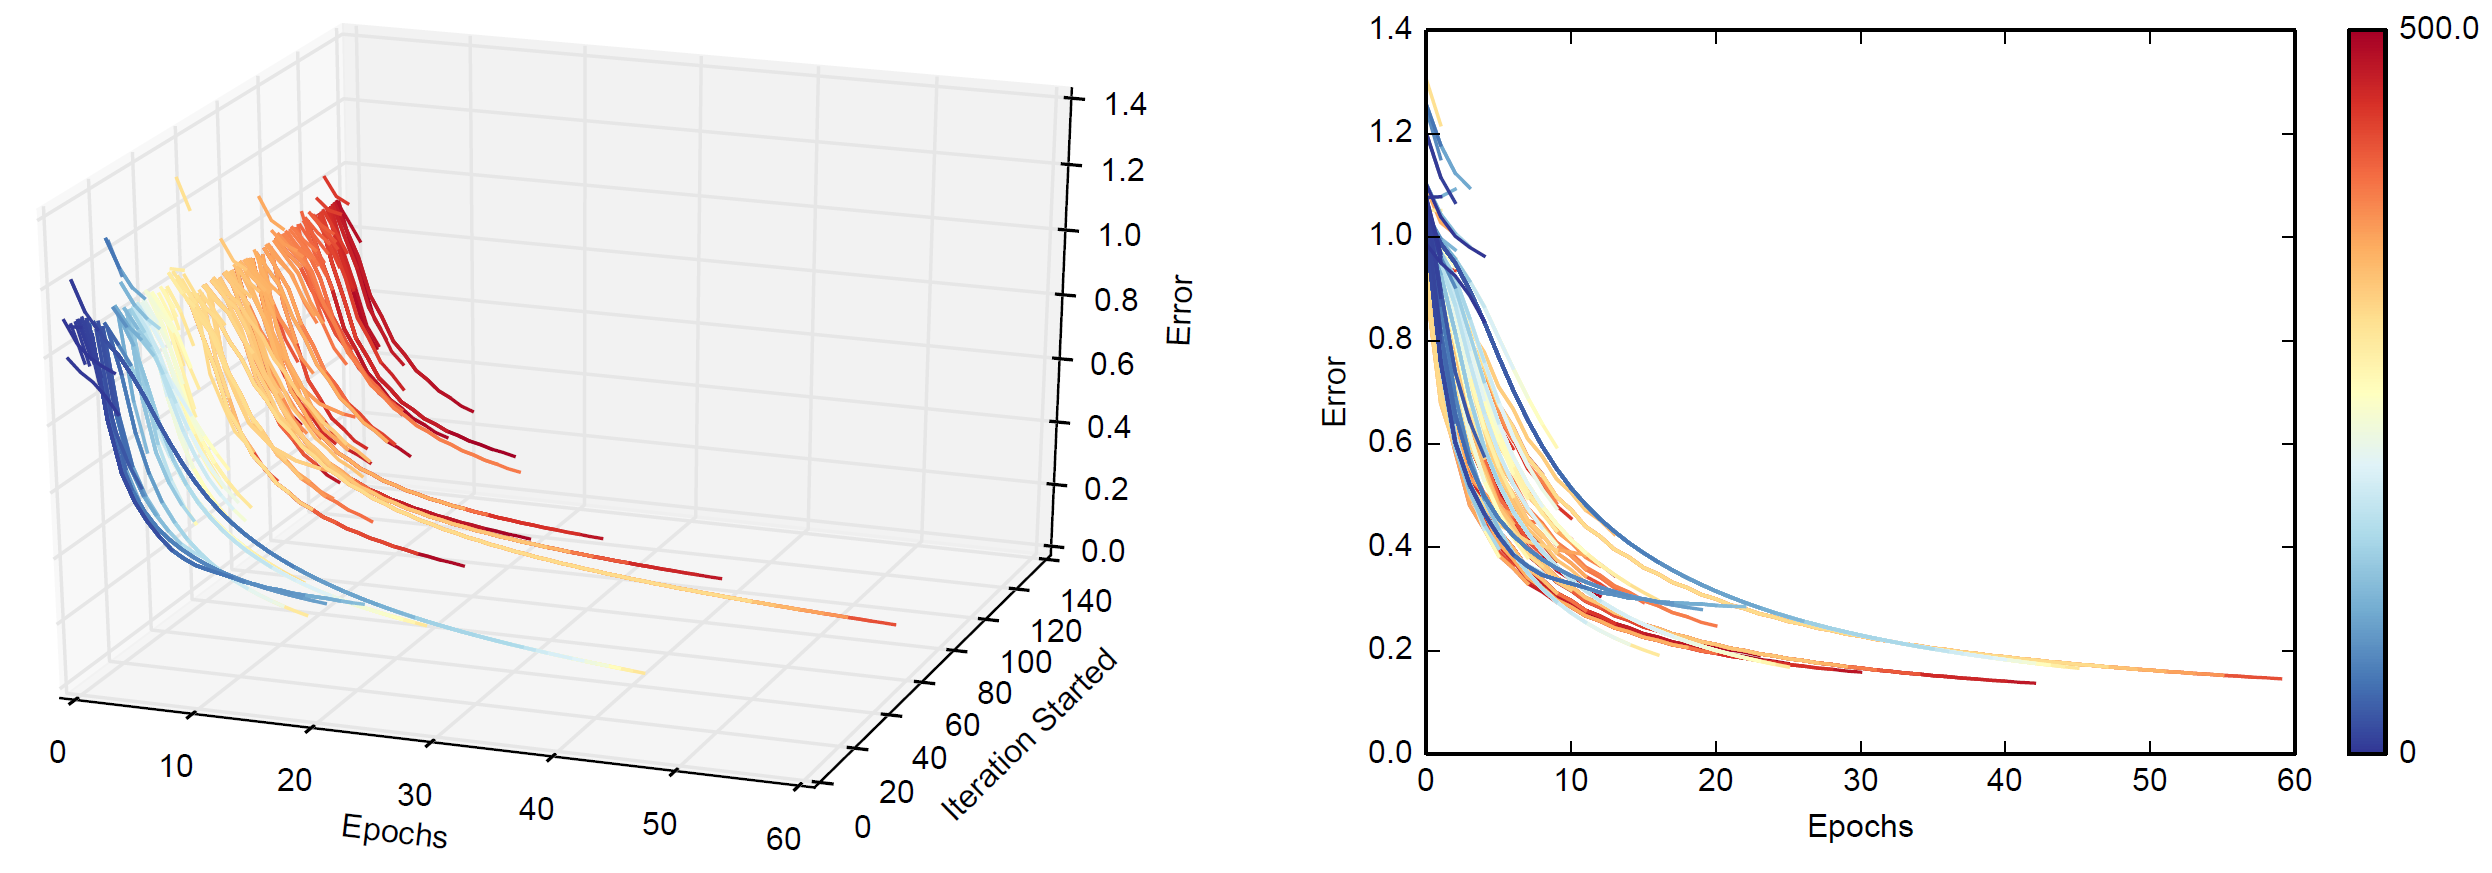
\includegraphics[width=0.8\textwidth]{w07_hpo_grey_box/images/learningcurve/FTBO.png}
\pause
	\item Unfortunately, no results for DNNs; no code available
}


\end{frame}
%-----------------------------------------------------------------------


%-----------------------------------------------------------------------
\begin{frame}{LC-Net}

\vspace*{-0.25em}
{
	\rightimage[.4]{w07_hpo_grey_box/images/learningcurve/LC-Net-network.png}
	\myit{
		\item \goleft[.45]{Make a layer out of the parametric learning curves by Domhan et al.}
		\item \goleft[.45]{Also support hyperparameters as inputs (in the figure denoted by $x_1, \dots, x_d$)}
%		\item \goleft[.45]{Work by my Phd student Aaron Klein and postdoc Stefan Falkner}
	}
}

\pause
\myit{
	\item Disadvantages of this model?
	\pause
	\myit{
		\item \goleft[.45]{Relies on manually-selected parametric families of curves}
		\item \goleft[.45]{Cannot quickly integrate new information from extending the current curve \\ (or from new runs)}
	}
}
\end{frame}
%-----------------------------------------------------------------------



%-----------------------------------------------------------------------
\begin{frame}{Sequence Models {\smaller{(e.g., Bayesian RNN)}}}

	\myit{
		\item Learning curves are \alert{sequences}
		\myit{
			\item Previous models don't treat them like this
			\item We can use an RNN (in particular, an LSTM) to predict the next value from a given sequence
			\item We can use variational dropout to obtain uncertainty estimates:
\pause
		}
	}

\begin{center}
	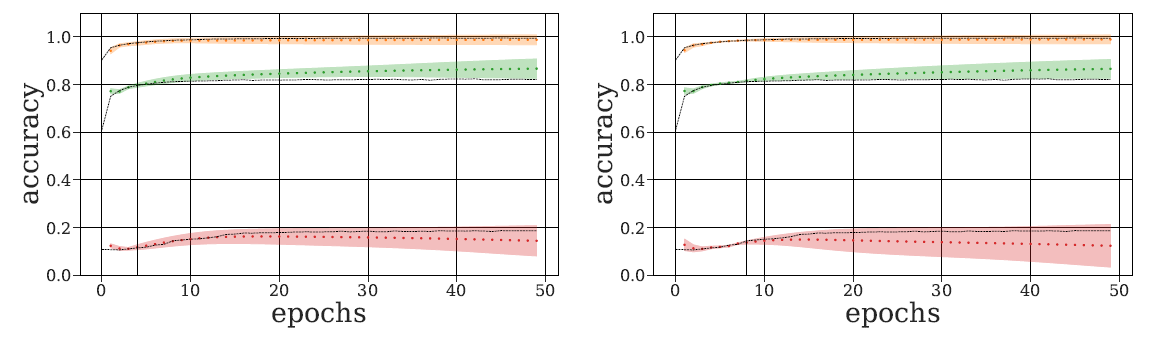
\includegraphics[width=0.58\textwidth]{w07_hpo_grey_box/images/learningcurve/Gargiani-MNIST-extrapolations_1.png}\\
	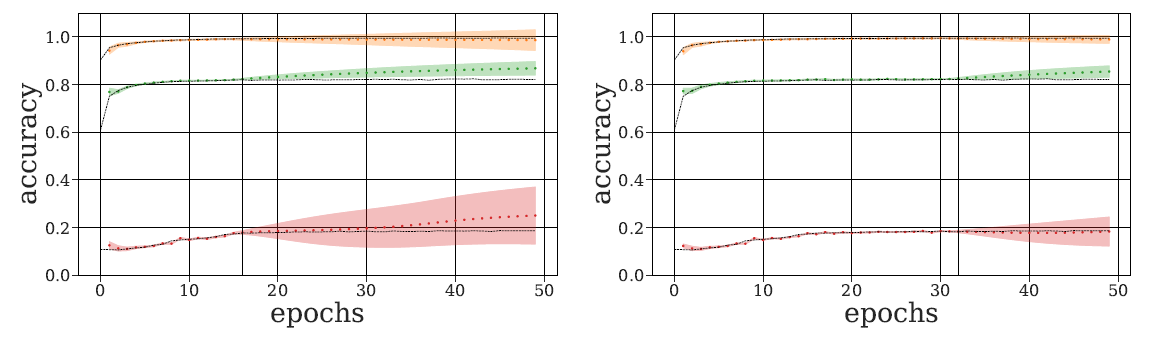
\includegraphics[width=0.58\textwidth]{w07_hpo_grey_box/images/learningcurve/Gargiani-MNIST-extrapolations_2.png}\\
\end{center}	
	
\end{frame}
%-----------------------------------------------------------------------
%-----------------------------------------------------------------------
\begin{frame}{Sequence Models {\smaller{(e.g., Bayesian RNN)}}}

	\myit{
		\item Note: we can also use a simpler model
		\myit{
			\item E.g., a random forest to map from a fixed-size window to the next value
		}
	}
\begin{center}
	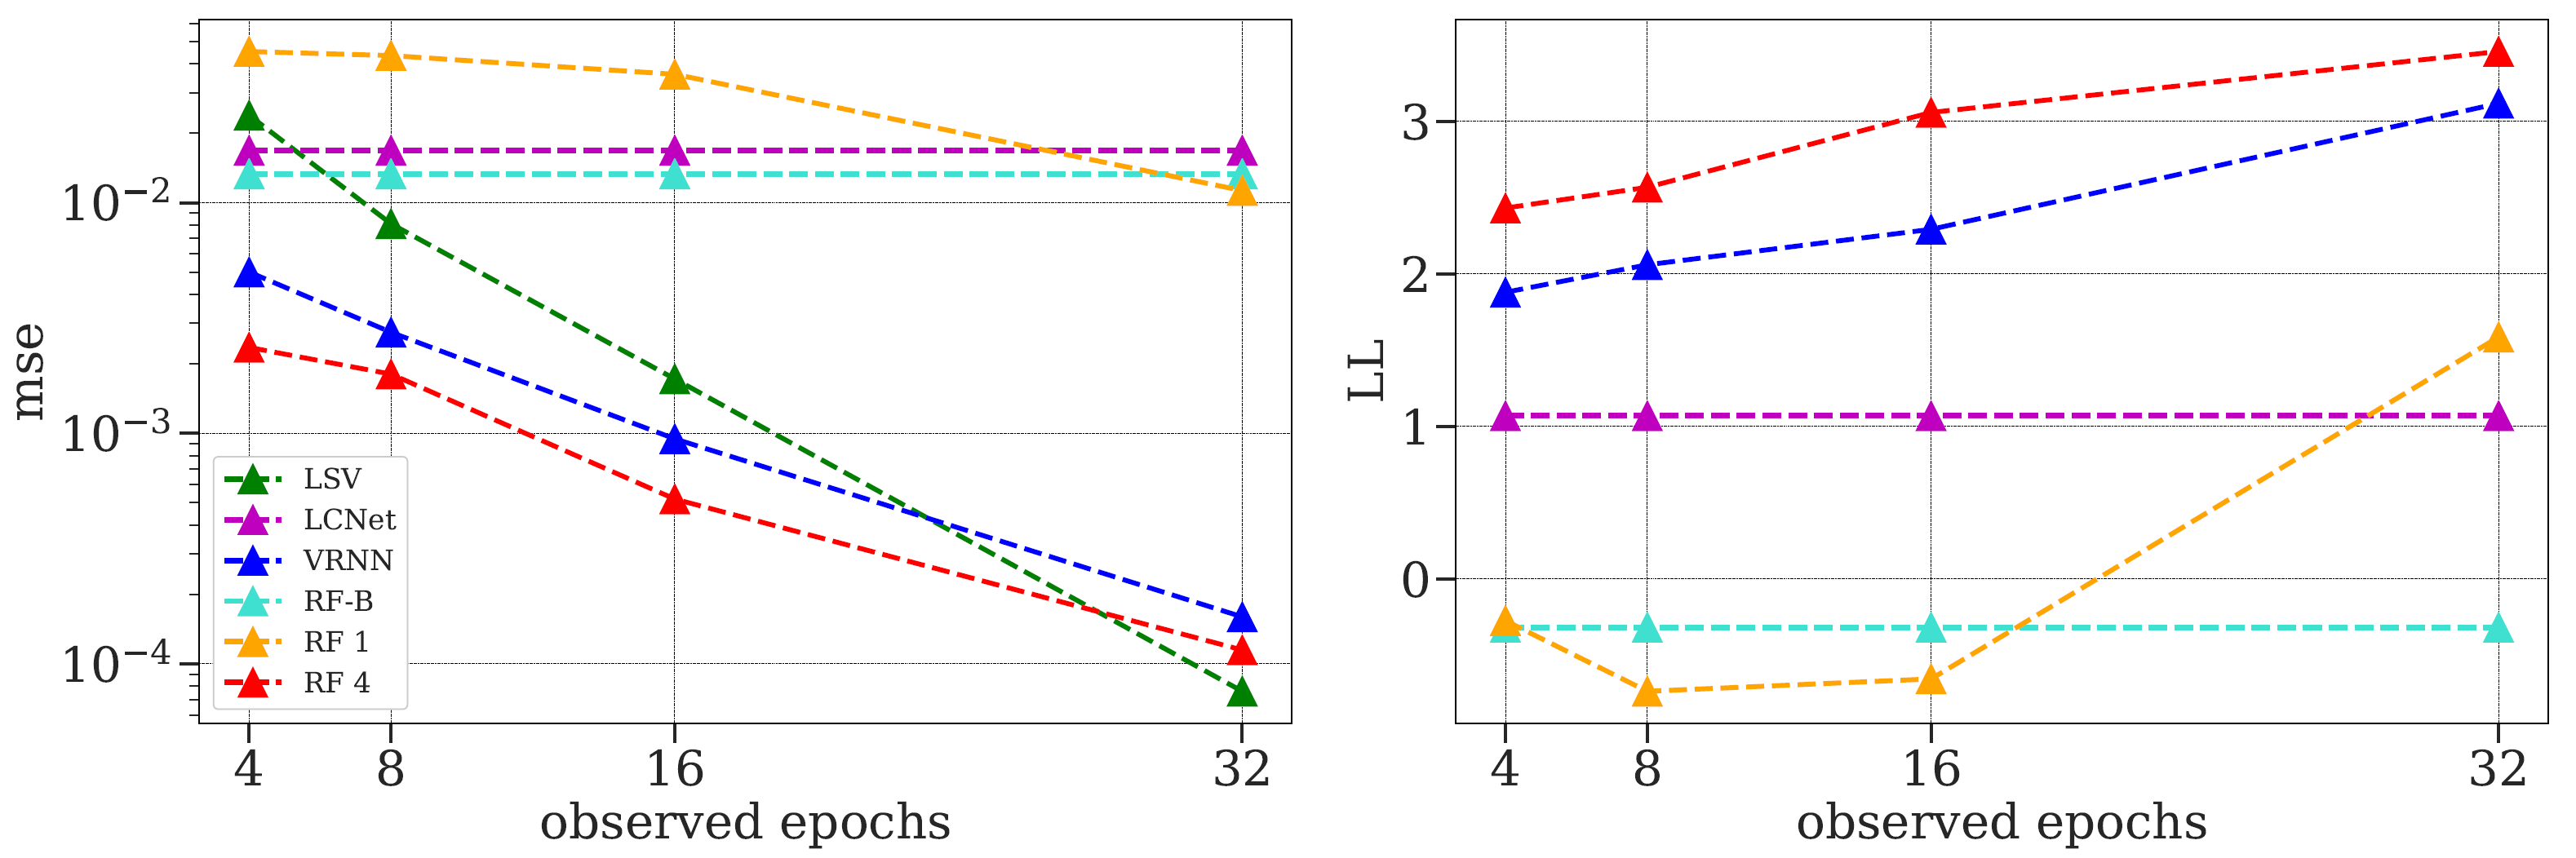
\includegraphics[width=0.9\textwidth]{w07_hpo_grey_box/images/learningcurve/Gargiani-MNIST-extrapolation-quality-based-on-different-sized-prefixes.png}
\end{center}	
\end{frame}
%-----------------------------------------------------------------------
%-----------------------------------------------------------------------
\begin{frame}{Compare: Baker et al, 2017}

	\myit{
		\item Idea: Map from configurations (including architectural hyperparameters) 
		and partial learning curves to the final performance

		\item Advantages
		\myit{
			\item \alert{Much simpler idea} than all the approaches just discussed: no need to model the entire learning curve
			\item \alert{Much easier to implement}
		}
		\item Disadvantage? \pause
		\alert{$\rightarrow$ requires many (e.g., 100) fully-evaluated learning curves as training data}
		\myit{
			\item After 100 full function evaluations we want to be pretty much converged in practice
			\item But definitely helpful for speeding up RL
			
		}
	}

%Describe simple idea, and how that works extremely well when you have a budget of 10.000 of function evaluations.

\end{frame}
%-----------------------------------------------------------------------


\myframe{Possible extension of LC models waiting to be done}{
	\myit{
		\item We could keep track of additional information to feed to our model for better predictions
		\myit{
			\item E.g., training \& validation cross-entropy loss \& accuracy
			\myit{
				\item Instead of only validation accuracy
			}
			\item E.g., split cross-entry into data-dependent \& weight dependent parts
			\item E.g., keep track of gradient norms, activation statistics, \ldots
		}
		\item Information about learning rate (\& weight decay) at each step
		\begin{itemize}
		    \item Only Predictive termination leads to a practically usable algorithm
		\end{itemize}
		
	}
}